\section{RESEARCH RESULTS}

This section presents the experimental results obtained from various configurations of the 
neural network, including hyperparameter optimization, comparisons of training algorithms, 
and the performance of the hybrid learning algorithm. 

All experiments were evaluated using 
a 80(+ synthetic data)-10-10 train-validation-test split, with accuracy and loss on unseen data 
as the primary performance metrics.

Reproducibility of results was an early focus in the implementation of this study; given the same
seed and configuration, the model repeats the same results across all epochs. For this reason,
each trial of ten independent samples cycled, in order, through the following integers, [42, 43, 44, 45, 46, 47, 48, 49, 50, 51]
where the first integer was used as the global seed for the first sample, the second integer for the second sample, and so on.
This ensured that results were not repeated while also preserving the model's underlying configuration for experimental validity. 

Additionally, results from paired t-tests, ANOVA (Analysis of Variance) and Tukey-HSD (Honest Significant Difference) tests 
of statistical significance are provided to substantiate claims of configuration-superiority. When conducting tests of statistical 
significance, all variables except the independent variable were held constant according 
to the specification outlined in the experimental set-up section.

Paired t-tests are used to compare the means of two related groups, typically 
measuring the same subjects before and after the independent variable is modified. It calculates the difference
 between each pair of observations and assesses whether the mean difference is significantly different 
 from zero. The test produces a t-statistic ($t_{stat}$), which measures the size of the difference relative to the 
 variability in the data. A p-value is then derived to determine whether the observed difference is likely 
 due to chance, with a p-value below a chosen threshold (in this study, $\alpha$ = 0.5) indicating a significant difference 
 between the paired groups.

The ANOVA test is used to determine if there are significant 
differences between the means of three or more groups. It calculates an F-statistic, which is the ratio 
of the variance between group means to the variance within groups, indicating how much the group means 
differ relative to random variation. A higher F-statistic suggests greater differences between groups. 
The p-value measures the probability that the observed differences occurred by chance, and if it is below 
a chosen significance level ($\alpha$ = $0.5$), the null hypothesis of equal means is rejected
and we conclude that the differences observed are statistically significant.

The Tukey-HSD test is a post-hoc analysis (used after an initial statistical test) that is applied after ANOVA to 
identify which specific group means are significantly different from each other. It calculates the mean differences 
between pairs of groups and compares them to a critical value, accounting for multiple pairwise comparisons and 
controlling for Type I error (incorrectly rejecting a true null hypothesis). A larger difference than the critical 
value indicates a significant difference between those group means. The test provides adjusted p-values for each 
comparison to control the family-wise error rate (FWER - the probability of making at least one Type I error), 
helping ensure the results are statistically valid. 

The {\sl meandiff} column shows the difference in means 
between two groups, while {\sl p-adj} is the adjusted p-value accounting for multiple comparisons, indicating the 
significance of the observed difference. The {\sl lower} and {\sl upper} columns provide the bounds of the confidence interval, 
showing the range within which the true mean difference likely falls. Together, these values assess the statistical 
significance and precision of the mean difference between groups.

\subsection{Grid Search: Number of Epochs by Learning Rate}

Preliminary tests identified the ranges $\eta$ = $[0.004, 0.1]$ and 
number of epochs = $[450, 750]$ as being worth further investigation via a grid-search. 

K-fold validation was used with $k$ = $3$ and involved splitting the dataset into three equal folds. During the grid-search the
model was trained on two of these folds in addition to all 20,000 rows of synthetic data and tested on the remaining fold. Each 
of the three independent runs on a configuration used a different rotation of the three folds.

The following plot visualizes the mean validation accuracies obtained across three independent runs for all 
49 ($\eta \, \times$ number of epochs) pairs where the total number of simulations conducted for the grid search was 147:

\noindent
\begin{figure}[thpb]
    \centering
    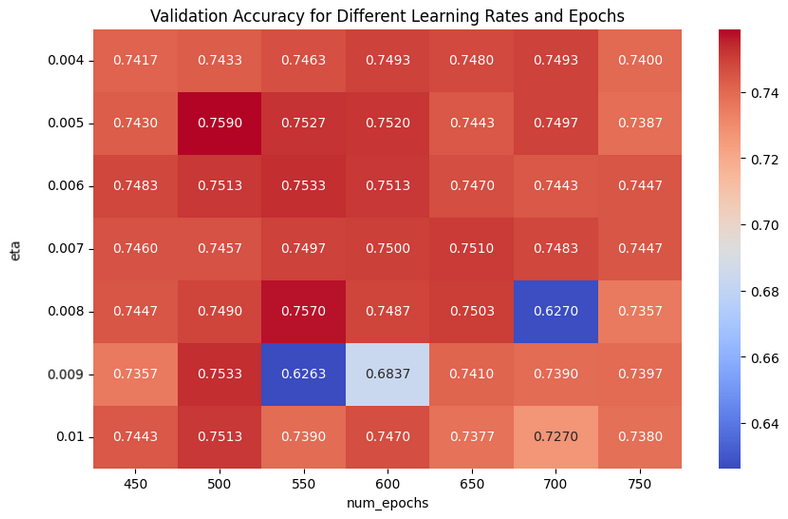
\includegraphics[scale=0.35]{img/grid-search.png}
    \caption{Grid search: mean results on accuracy of three independent runs per configuration.}
\end{figure}

The grid-search results highlighted several promising configurations whereafter the epoch range $[550,600]$ was investigated.
After further cross-validation and fine-tuning of the model, the highest accuracy was observed using 600 epochs with $\eta$ = 0.007.

\subsection{Dropout Usage}

The usage of dropout applied to each hidden layer, with probability of dropout $p$ = 0.5, and its effect on the model's performance was tested using a paired t-test ($\alpha$ = 0.05). 

The mean accuracy achieved when dropout was {\sl enabled} was $0.644$ ($\sigma$ = $0.018$) with a mean loss of $0.784$ ($\sigma$ = $ 0.019$). 

The mean accuracy achieved when dropout was {\sl disabled} was $0.757$ ($\sigma$ = $0.02$) with a mean loss of $0.628$ ($\sigma$ = $0.048$).

The paired t-test results on accuracy ($t_{\text{stat}}$ = $-12.547$, p-value = $5.261 \times 10^{-7}$) indicate that there is
 a significant difference between the accuracies observed when dropout was enabled versus when it was disabled.

The paired t-test results on loss ($t_{\text{stat}}$ = $8.192$, 
p-value = $1.831 \times 10^{-5}$), indicate that there is a significant difference between the losses observed when dropout was 
enabled versus when it was disabled.

Therefore, for this study's implementation, using dropout significantly diminished the model's
performance on unseen almond-cases in terms of accuracy and loss. 

\subsection{Batch Size}

The model was tested using three batch-size configurations—32, 64, and 128. The observed performance metrics are as follows: \\

\noindent
\footnotesize
\setlength{\tabcolsep}{6pt} % Adjusts padding (slightly larger)
\renewcommand{\arraystretch}{1.0} % Adjusts row height (slightly larger)
\begin{center}
\begin{tabular}{l|cc|cc}
\toprule
\textbf{Batch Size} & \multicolumn{2}{c|}{\textbf{Accuracy}} & \multicolumn{2}{c}{\textbf{Loss}} \\
\cmidrule(r){2-3} \cmidrule(l){4-5}
 & $\mu$ & $\sigma$ & $\mu$ & $\sigma$ \\
\midrule 
32   & 0.757 & 0.020 & 0.628 & 0.048 \\
64   & 0.776 & 0.014 & 0.564 & 0.040 \\
128  & 0.780 & 0.013 & 0.531 & 0.022 \\
\bottomrule
\end{tabular}
\end{center}

\normalsize

\vspace{0.7em}

The ANOVA results on accuracy ($F$-stat = $5.229$, p-value = $0.012$) indicate that there is a significant 
difference between the observed accuracies between the batch-sizes.

The Tukey-HSD (FWER = $0.05$) results on accuracy are as follows: \\

\noindent
\resizebox{\linewidth}{!}{%
\begin{tabular}{ccccccc}
\toprule
Batch Size 1 & Batch Size 2 & Mean Diff & p-adj  & Lower   & Upper   & Reject \\
\midrule
32 & 64 & 0.0189    & 0.0465 & 0.0003  & 0.0375  & True   \\
32 & 128 & 0.0227    & 0.0147 & 0.0041  & 0.0413  & True   \\
64 & 128 & 0.0038    & 0.8694 & -0.0148 & 0.0224  & False  \\
\bottomrule
\end{tabular}%
} \\

These results indicate that there are significant differences in the observed accuracies between batch-sizes 32 and 64, and between 32 and 128 but no significant difference
between batch-sizes 64 and 128.

The ANOVA results on losses ($F$-stat = $14.836$, p-value = $4.497 \times 10^{-5}$)
indicate that there is a significant difference between the observed losses between the batch-sizes.

The Tukey-HSD (FWER = $0.05$) results on losses are as follows: \\

\noindent
\resizebox{\linewidth}{!}{%
\begin{tabular}{ccccccc}
\toprule
Batch-Size 1 & Batch-Size 2 & Mean Diff & p-adj  & Lower   & Upper   & Reject \\
\midrule
32 & 64 & -0.0633   & 0.0044 & -0.1080 & -0.0186 & True   \\
32 & 128 & -0.0967   & 0.0    & -0.1414 & -0.0520 & True   \\
64 & 128 & -0.0334   & 0.1722 & -0.0781 & 0.0113  & False  \\
\bottomrule
\end{tabular}%
} \\

The Tukey-HSD results indicate that there were significant differences in loss between batch-sizes 32 and 64, and between 32 and 128 but no significant difference
between batch-sizes 64 and 128.

\subsection{Weight Initialization}

Two built-in PyTorch weight initialization strategies were tested, namely He-Kaiming uniform 
and Xavier uniform. He-Kaiming initializes weights to values sampled from a uniform distribution 
scaled by the inverse square root of the number of input units, optimized for ReLU activations. 
Xavier uniform initializes weights to values sampled from a uniform distribution scaled by the 
inverse square root of the sum of input and output units, optimized for sigmoid or hyperbolic-tangent (tanh) activations.

Both strategies were tested in isolation using a paired t-test ($\alpha = 0.05$) to assess the statistical significance of their effect on the
model's performance.

The mean accuracy achieved when using Xavier uniform was $0.757$ ($\sigma = 0.02$) with a mean loss of $0.628$ ($\sigma$ = $0.0048$). 

The mean accuracy achieved when using He-Kaiming uniform was $0.768$ ($\sigma = 0.017$) with a mean loss of $0.607$ ($\sigma$ = $0.07$)

The paired t-test results on accuracies ($t_{\text{stat}}$ = $-1.029$, 
p-value $= 0.331$) indicate that there is no significant difference between the observed accuracies.

The paired t-test results on losses ($t_{\text{stat}}$ = $0.749$, 
p-value $= 0.473$) indicate that there is no significant difference between the observed losses.

\subsection{Hybrid-Learning}

A comparison of the RProp, Adam, and RMSProp training algorithms was conducted to determine the performance effects
of using each algorithm individually. The observed performance metrics are as follows: \\

\noindent
\footnotesize
\setlength{\tabcolsep}{6pt} % Adjusts padding (slightly larger)
\renewcommand{\arraystretch}{1.0} % Adjusts row height (slightly larger)
\begin{center}
\begin{tabular}{l|cc|cc}
\toprule
\textbf{Algorithm} & \multicolumn{2}{c|}{\textbf{Accuracy}} & \multicolumn{2}{c}{\textbf{Loss}} \\
\cmidrule(r){2-3} \cmidrule(l){4-5}
 & $\mu$ & $\sigma$ & $\mu$ & $\sigma$ \\
\midrule 
Adam   & 0.776 & 0.014 & 0.564 & 0.040 \\
RProp  & 0.601 & 0.024 & 0.872 & 0.024 \\
RMSProp & 0.776 & 0.013 & 0.552 & 0.036 \\
\bottomrule
\end{tabular}
\end{center}

\normalsize

\vspace{0.7em}

The ANOVA results on accuracies ($F$-stat = $297.998$, p-value = $3.961 \times 10^{-19}$) 
indicate that there is a significant difference between the accuracies observed.

The Tukey-HSD (FWER = $0.05$) results on accuracy are as follows: \\

\noindent
\resizebox{\linewidth}{!}{%
\begin{tabular}{ccccccc}
\toprule
Group 1 & Group 2 & Mean Diff & p-adj  & Lower   & Upper   & Reject \\
\midrule
Adam & RProp & -0.1747   & 0.0    & -0.1952 & -0.1542 & True   \\
Adam & RMSProp & 0.0003    & 0.9993 & -0.0202 & 0.0208  & False  \\
RProp & RMSProp & 0.1750    & 0.0    & 0.1545  & 0.1955  & True   \\
\bottomrule
\end{tabular}%
} \\

The Tukey-HSD results on accuracies indicate that a significant difference in accuracy exists between Adam and RProp, and between RMSProp and RProp but not between
Adam and RMSProp.

The ANOVA results on losses
($F$-stat = $256.021$, p-value = $2.795 \times 10^{-18}$) indicate that there is a significant difference between losses observed.

The Tukey-HSD (FWER = $0.05$) results on losses are as follows: \\

\noindent
\resizebox{\linewidth}{!}{%
\begin{tabular}{ccccccc}
\toprule
Group 1 & Group 2 & Mean Diff & p-adj  & Lower   & Upper   & Reject \\
\midrule
Adam & RProp & 0.3072    & 0.0    & 0.2675  & 0.3469  & True   \\
Adam & RMSProp & -0.0125   & 0.7177 & -0.0522 & 0.0272  & False  \\
RProp & RMSProp & -0.3197   & 0.0    & -0.3594 & -0.2800 & True   \\
\bottomrule
\end{tabular}%
} \\

The Tukey-HSD results on losses indicate that significant differences in loss exist between 
Adam and RProp, and between RMSProp and RProp but not between Adam and RMSProp.

Then, a hybrid-learning implementation was used to compare RProp, Adam, and RMSProp in pairs. The observed performance metrics
are as follows: \\

\noindent
\footnotesize
\setlength{\tabcolsep}{6pt}
\renewcommand{\arraystretch}{1.0}
\begin{center}
\begin{tabular}{l|cc|cc}
\toprule
\textbf{Algorithm Pair} & \multicolumn{2}{c|}{\textbf{Accuracy}} & \multicolumn{2}{c}{\textbf{Loss}} \\
\cmidrule(r){2-3} \cmidrule(l){4-5}
 & $\mu$ & $\sigma$ & $\mu$ & $\sigma$ \\
\midrule 
RProp + RMSProp   & 0.778 & 0.013 & 0.542 & 0.024 \\
Adam + RMSProp   & 0.767 & 0.016 & 0.599 & 0.444 \\
RProp + Adam   & 0.784 & 0.018 & 0.534 & 0.034 \\
\bottomrule
\end{tabular}
\end{center}

\normalsize

\vspace{0.7em}

The ANOVA results on accuracy ($F$-stat = $2.862$, p-value = $0.075$) indicate that there is no significant difference between the observed accuracies.

The Tukey-HSD (FWER = $0.05$) results on accuracy are as follows: \\

\noindent
\resizebox{\linewidth}{!}{
\begin{tabular}{ccccccc}
\toprule
Group 1 & Group 2 & Mean Diff & p-adj & Lower & Upper & Reject \\
\midrule
RProp + RMSProp  & Adam + RMSProp & -0.0115   & 0.2924 & -0.0301 & 0.0071  & False \\
RProp + RMSProp  & RProp + Adam   & 0.0062    & 0.6905 & -0.0124 & 0.0248  & False \\
Adam + RMSProp   & RProp + Adam   & 0.0177    & 0.0647 & -0.0009 & 0.0363  & False \\
\bottomrule
\end{tabular}
} \\

The Tukey-HSD results on accuracies reiterate the findings of the ANOVA test, namely that no significant 
difference exists between the mean observed accuracies.

The ANOVA results on losses ($F$-stat = $9.314$, p-value = $0.00084$) indicate that a 
significant difference exists between the losses observed.

The Tukey-HSD (FWER = $0.05$) results on losses are as follows: \\

\noindent
\resizebox{\linewidth}{!}{%
\begin{tabular}{ccccccc}
\toprule
Pair 1 & Pair 2 & Mean Diff & p-adj & Lower   & Upper  & Reject \\
\midrule
RProp + RMSProp  & Adam + RMSProp & 0.0573    & 0.0048 & 0.0164  & 0.0982  & True \\
RProp + RMSProp  & RProp + Adam   & -0.0079   & 0.8817 & -0.0488 & 0.033   & False \\
Adam + RMSProp   & RProp + Adam   & -0.0652   & 0.0014 & -0.1061 & -0.0243 & True \\
\bottomrule
\end{tabular}%
} \\

The Tukey-HSD results indicate that there is a significant difference between the losses of [{\sl RProp}, {\sl RMSProp}] and [{\sl Adam}, {\sl RMSProp}],
that no significant difference exists between the losses of [{\sl RProp}, {\sl RMSProp}] and [{\sl RProp}, {\sl Adam}] and that there was a significant
difference between the losses of [{\sl Adam}, {\sl RMSProp}], and [{\sl RProp}, {\sl Adam}].

According to these results, [{\sl Adam}, {\sl RMSProp}] performs the worst in this study's hybrid-learning implementation.

Finally, a comparison is made between the individual performance effects of the individual training algorithms versus their 
effects when used in hybrid-learning pairs.

The ANOVA results on accuracy between the six test groups
($F$-stat = $164.712$, p-value = $2.085 \times 10^{-31}$) indicate that there is a significant difference between the 
mean observed accuracies.

The Tukey-HSD (FWER = $0.05$) results on accuracy are as follows: \\

\noindent
\resizebox{\linewidth}{!}{%
\begin{tabular}{ccccccc}
\toprule
Group 1 & Group 2 & Mean Diff & p-adj  & Lower   & Upper   & Reject \\
\midrule
Adam & R + RMS & 0.0022    & 0.9998 & -0.0211 & 0.0255  & False  \\
Adam & A + RMS & -0.0093   & 0.8455 & -0.0326 & 0.0140  & False  \\
Adam & R + A & 0.0084    & 0.8935 & -0.0149 & 0.0317  & False  \\
RProp & R + RMS & 0.1769    & 0.0    & 0.1536  & 0.2002  & True   \\
RProp & A + RMS & 0.1654    & 0.0    & 0.1421  & 0.1887  & True   \\
RProp & R + A & 0.1831    & 0.0    & 0.1598  & 0.2064  & True   \\
RMSProp & R + RMS & 0.0019    & 0.9999 & -0.0214 & 0.0252  & False  \\
RMSProp & A + RMS & -0.0096   & 0.8274 & -0.0329 & 0.0137  & False  \\
RMSProp & R + A & 0.0081    & 0.9073 & -0.0152 & 0.0314  & False  \\
\bottomrule
\end{tabular}%
} \\

The Tukey-HSD results indicate that a significant improvement in accuracy was gained by using any of the investigated hybrid-learning pairs when compared
to the performance when using the RProp training algorithm alone.

By the ANOVA results on losses between the six groups, we reject the null hypothesis ($F$-stat = $127.851$, p-value = $1.181 \times 10^{-28}$), i.e. 
there is a significant difference between the 
mean losses observed between pairs of training algorithms and individually-used training algorithms.

The Tukey-HSD (FWER = $0.05$) results on losses are as follows: \\

\noindent
\resizebox{\linewidth}{!}{%
\begin{tabular}{ccccccc}
\toprule
Group 1 & Group 2 & Mean Diff & p-adj  & Lower   & Upper   & Reject \\
\midrule
Adam & R + RMS & -0.0224   & 0.7394 & -0.0704 & 0.0256  & False  \\
Adam & A + RMS & 0.0349    & 0.2791 & -0.0131 & 0.0829  & False  \\
Adam & R + A & -0.0303   & 0.4345 & -0.0783 & 0.0177  & False  \\
RProp & R + RMS & -0.3296   & 0.0    & -0.3776 & -0.2816 & True   \\
RProp & A + RMS & -0.2723   & 0.0    & -0.3203 & -0.2243 & True   \\
RProp & R + A & -0.3375   & 0.0    & -0.3855 & -0.2895 & True   \\
RMSProp & R + RMS & -0.0099   & 0.9899 & -0.0579 & 0.0381  & False  \\
RMSProp & A + RMS & 0.0474    & 0.0548 & -0.0006 & 0.0954  & False  \\
RMSProp & R + A & -0.0178   & 0.8811 & -0.0658 & 0.0302  & False  \\
\bottomrule
\end{tabular}%
} \\

The Tukey-HSD results indicate that a significant reduction in loss occurred when using any of the investigated hybrid-learning pairs when compared
to the performance of using the RProp training algorithm alone.

\subsection{Data Augmentation}

20,000 sythetic rows of additional training data were generated to augment the original almond dataset of 2,803 rows. The performance effects 
of incorporating the synthetic data during training were tested via the ANOVA and Tukey-HSD statistical significance tests. The observed performance
metrics are as follows: \\

\noindent
\footnotesize
\setlength{\tabcolsep}{6pt} % Adjusts padding (slightly larger)
\renewcommand{\arraystretch}{1.0} % Adjusts row height (slightly larger)
\begin{center}
\begin{tabular}{l|cc|cc}
\toprule
\textbf{Synthetic Utilisation} & \multicolumn{2}{c|}{\textbf{Accuracy}} & \multicolumn{2}{c}{\textbf{Loss}} \\
\cmidrule(r){2-3} \cmidrule(l){4-5}
 & $\mu$ & $\sigma$ & $\mu$ & $\sigma$ \\
\midrule 
0 (0\%)     & 0.742 & 0.023 & 0.779 & 0.074 \\
10,000 (50\%) & 0.765 & 0.017 & 0.651 & 0.064 \\
20,000 (100\%) & 0.776 & 0.014 & 0.564 & 0.040 \\
\bottomrule
\end{tabular}
\end{center}

\normalsize

\vspace{0.7em}

The ANOVA results on accuracy ($F$-stat = $8.227$, p-value = $0.001$) indicate that there is a significant difference 
between the observed accuracies.

The Tukey-HSD (FWER = $0.05$) results on accuracy are as follows: \\

\noindent
\resizebox{\linewidth}{!}{%
\begin{tabular}{ccccccc}
\toprule
Util. 1 & Util. 2 & Mean Diff & p-adj & Lower   & Upper  & Reject \\
\midrule
0\% & 50\% & 0.023    & 0.0325 & 0.0017  & 0.0443  & True \\
0\% & 100\% & 0.0342   & 0.0013 & 0.0129  & 0.0555  & True \\
50\% & 100\% & 0.0112   & 0.4059 & -0.0101 & 0.0325  & False \\
\bottomrule
\end{tabular}%
} \\

The Tukey-HSD results on accuracy indicate that there is a significant difference in accuracies observed when using none of the synthetic data
versus using half of the synthetic data. 

The results also indicate that there is a significant difference in observed accuracies between using half of the synthetic
data versus using all 20,000 rows. 

However, no significant difference exists in accuracy between when the training set is augmented with half of the synthetic data
versus when the training set is augmented with all of the synthetic data. This is useful information because training a model on ~10,000 rows
of CSV data is far less computaionally expensive than training a model on ~20,000 rows of CSV data.

The ANOVA results on loss,
($F$-stat = $33.794$, p-value = $4.463 \times 10^{-8}$) indicate that there is a significant difference between 
the observed losses.

The Tukey-HSD (FWER = $0.05$) results are as follows: \\

\noindent
\resizebox{\linewidth}{!}{%
\begin{tabular}{ccccccc}
\toprule
Util. 1 & Util. 2 & Mean Diff & p-adj  & Lower   & Upper   & Reject \\
\midrule
0\% & 50\% & -0.1482   & 0.0001 & -0.2197 & -0.0767 & True   \\
0\% & 100\% & -0.2342   & 0.0    & -0.3057 & -0.1627 & True   \\
50\% & 100\% & -0.0860   & 0.0159 & -0.1575 & -0.0145 & True   \\
\bottomrule
\end{tabular}%
} \\

The Tukey-HSD results on observed losses indicate that there is a significant difference in losses observed when using none of the synthetic data
versus half of the synthetic data. They also indicate that there is a significant difference in losses observed when using half of the synthetic
data versus all. 

However, there is no significant difference in loss between when the training set is augmented with half of the synthetic data
versus when the training set is augmented with all of the synthetic dataset.

\subsection{Learning Rate Scheduler}

The model was tested using three learning-rate scheduler configurations—a constant learning rate ($\eta$ = $0.007$), 
exponential decay, and CAWR. The observed performance metrics are as follows: \\

\noindent
\footnotesize
\setlength{\tabcolsep}{6pt} % Adjusts padding (slightly larger)
\renewcommand{\arraystretch}{1.0} % Adjusts row height (slightly larger)
\begin{center}
\begin{tabular}{l|cc|cc}
\toprule
\textbf{Learning Rate Schedule} & \multicolumn{2}{c|}{\textbf{Accuracy}} & \multicolumn{2}{c}{\textbf{Loss}} \\
\cmidrule(r){2-3} \cmidrule(l){4-5}
 & $\mu$ & $\sigma$ & $\mu$ & $\sigma$ \\
\midrule 
Constant ($\eta = 0.007$)  & 0.748 & 0.012 & 0.594 & 0.029 \\
Exponential Decay  & 0.748 & 0.011 & 0.599 & 0.011 \\
CAWR   & 0.757 & 0.020 & 0.628 & 0.048 \\
\bottomrule
\end{tabular}
\end{center}

\normalsize

\vspace{0.7em}


The ANOVA results on accuracy ($t_{\text{stat}} = 1.089$, 
p-value $= 0.351$) indicate that there is no significant difference between the observed accuracies.

The Tukey-HSD (FWER = $0.05$) results on accuracies are as follows: \\

\noindent
\resizebox{\linewidth}{!}{%
\begin{tabular}{ccccccc}
\toprule
LRS 1 & LRS 2 & Mean Diff & p-adj  & Lower   & Upper   & Reject \\
\midrule
Constant & Exp. & -0.0001   & 0.9999 & -0.0173 & 0.0171  & False  \\
Constant & CAWR & 0.0088    & 0.4232 & -0.0084 & 0.0260  & False  \\
Exp. & CAWR & 0.0089    & 0.4153 & -0.0083 & 0.0261  & False  \\
\bottomrule
\end{tabular}%
} \\


The Tukey-HSD results indicate that there are no significant differences in observed accuracies between the three learning-rate schedulers tested in this study.

The ANOVA results on losses ($t_{\text{stat}} = 2.784$, 
p-value = $0.082$) indicate that no significant differences exists between the observed losses.

The Tukey-HSD (FWER = $0.05$) results are as follows: \\

\noindent
\resizebox{\linewidth}{!}{%
\begin{tabular}{ccccccc}
\toprule
LRS 1 & LRS 2 & Mean Diff & p-adj  & Lower   & Upper   & Reject \\
\midrule
Constant & Exp. & 0.0055    & 0.9329 & -0.0329 & 0.0439  & False  \\
Constant & CAWR & 0.0338    & 0.0921 & -0.0046 & 0.0722  & False  \\
Exp. & CAWR & 0.0283    & 0.1793 & -0.0101 & 0.0667  & False  \\
\bottomrule
\end{tabular}%
} \\

The Tukey-HSD results indicate that there are no significant differences in observed losses between any of the learning-rate schedulers when tested in this study.

\subsection{Key Findings}

The highest accuracy achieved on unseen test data was 82.2\% with a loss of 0.49. Notably, training loss was higher 
than validation loss and validation loss higher than test loss when all 20,000 rows of synthetic data were added to the training set.

\begin{figure}[thpb]
    \centering
    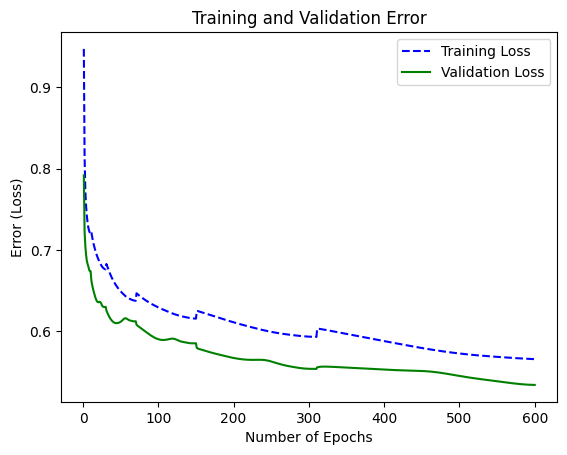
\includegraphics[scale=0.4]{img/loss.png}
    \caption{Loss by Number of Epochs on Best Run}
\end{figure}

A reason for this may
be because the synthetic data introduced noise that the model struggled to generalize during training, leading to overfitting on the 
training set but improved performance on the unseen validation and test sets due to the added diversity of the additional data.
